\section*{Approach}

\section{Aim 1}

\subsection{Rationale}

In the first step of Aim 1, the fabrication process of the TCP will be developed to a point of consistency in for testing. Once this process is proven to be consistent and reliable, the next steps will be modeling the system, and choosing a control architecture which can maintain a consistent configuration of the TCP with little-to-no error.

In order to achieve a consistent fabrication process, the TCP will be spun using an automated system; similar to that of a rope making machine. The system will be configurable to a set number of rotations, and a set RPM speed, as well as having connections for an adjustable counter-weight which will be used as the third and final configuration input when making the material. Once the fabrication process is created and checked for consistency, data will be collected on the actuation capabilities of the string with varying configuration inputs. A setup will be chosen based on the parameters collected.

The next step is to derive a control model formula which can represent the tension exhibited by a single strand of the TCP with inputs set to current and voltage. The constant parameters of the system will ideally be the same as the parameters used when creating the TCP string, but will require more testing to legitimize. Because TCP is actuated via heat generation, the system dynamics will be time-dependent, and will be discussed in the next section.

Finally, a controller will be implemented (figure \ref{fig:control_diagram}), ideally using the aforementioned model formula. The current plan is to utilize a control architecture similar to model predictive control (MPC) which would create the most accurate system available. MPC, and its alternatives will be more thoroughly discussed in the next section.

\begin{figure}[ht]
	\centering
	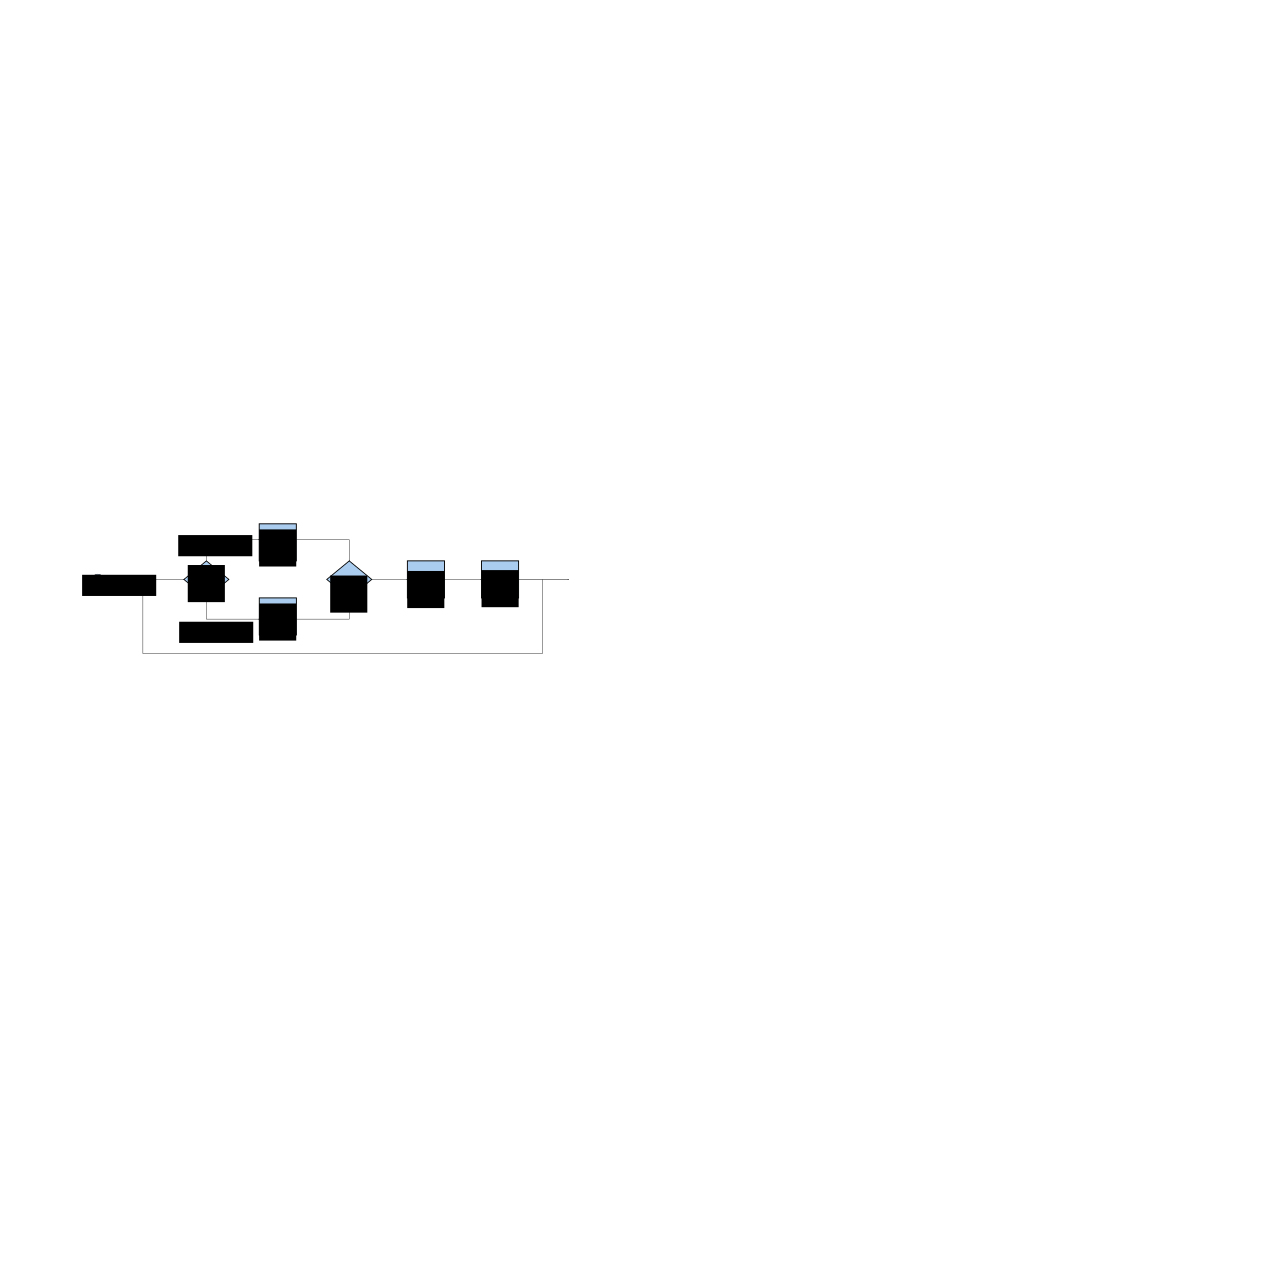
\includegraphics[scale=0.30]{control_diagram}
	\caption{AEI System Control Diagram}
	\label{fig:control_diagram}
\end{figure}

\subsection{Approach}

The fabrication of the TCP material will be facilitated through an in-house rope making machine which are standard and can be automated relatively easily. The wire of choise will be silver-coated nylon 66 wire, similar to that used in the initial prototype. The control board of choice for the automation will be an Arduino Uno, and will be used to control the RPM of the machine, as well as the number of spins. The counter-weight attached to the machine can also be adjusted for further variations. For consistency, the length of the TCP created at a given time will be held constant, and will be heat-treated and trained using the research varified by [CITE SOURCE FOR FABRICATION].

Modeling of the TCP system will be the most difficult of the steps discussed in this research. Here, the formula for the TCP dynamics will be simplfied to take the inputs current and voltage, and output the tension created after a certain period of time. This is achieved in the research conducted here [CITE MODELING ARTICLE]. The model will be compared to the real TCP using a tension measurement device, and by holding the current and voltage constant over the intended period of time. In this way, the error between the model and the real system can be evaluated at varying configuration settings. With tension calculated, the system then be directly compared to a solely tension-driven actuation system. This effectively turns the model from a current (input) to tension (output) calculation, to a current (input) to motion (output) formula.

The controller for the system will ideally be model-dependent. It is understood that model-dependent controllers, when accurately tuned, create the most effective system controllers and are more reliable and robust then model-independent alternatives. Also, considering the time-dependence of the TCP system, the use of MPC will be prioritized because of its ability to look into future states and solve for the optimal set of inputs at a given point in time.

\subsection{Risks and Alternatives}

It is understood that all of the steps taken in this portion of the development process are subject to considerable obstacles. That said, each of the discussed approaches have alternative methods of attack which should still achieve the overarching goals of the project.

In the case of the fabrication. It is likely that the TCP string may be too thin, inconsistent string could be purchased, or the machine itself may be too intricate to make/program in-house. In the scenario of thin or inconsistent string, there are many companies that make the intended wire and ordering thicker/more consistent silver-coated polymer wire is possible. Once a certain brand of wire proves sifficient, it will be ordered in bulk and used for the remainder of the project. If the machine proves too inctricate to make by hand, it is also possible to order small scale rope making machines online.

Since TCP is a relatively new form of actuation and is time-dependent, verified methods of modelling are not easily found. Here, the equations derived from the research of Farzad Karami and Yonas Tadesse in [CITE MODELING ARTICLE] will be used to supplement the formulations found in-house. In the extreme case that the model cannot be derived analytically, it is also possible to train a neural network to produce the intended behavior. This would involve considerably more data on configuration details, but is very possible and has been done for likewise projects in the past [SE3-nets ARTICLE, YANG AND MENG ARTICLE].

\section{Aim 2}

\subsection{Rationale}

In aim 2, the design of the end effector, and the core tubing is addressed. In this portion of the project, the end effector will be designed to house the TCP such that it is not exposed, can be replaced when necessary, and does not limit its range of motion. To achieve this, the four strands of TCP will be lined in parallel to the center tube, which contains the ground wire, as well as the camera.

The core tubing which is extruded from the housing module, and connects to the end effector via a clip system will likewise need to house the necessary wires to the TCP, the ground wire, and the camera wiring. This portion of the tubing will be relatively simple in configuration, with the primary limiting factor being the diameter of the tube.

\subsection{Approach}

The end effector will be constructed with the intent of a two-layer configuration. The center will be comprised of the ground wire and the camera, similar to the prototype made during the OSU capstone project with an insulating tube surrounding the components (layer 1). Next, the TCP will be connected in parallel around the center shaft and connected to the common ground wire. Each string will also be connected to an individual active wire which is used to control the current supplied to the TCP from the main controller. The TCP will then be surrounded by another layer of insulated tubing (layer 2). It is also possible that a third intermediate layer will be introduced to insulate the individual TCP string from one another, this will hopefully be aavoidable though as it would unnecessarily increase the diamter of the assembled system. This portion of the device will only span one to two inches in length. Note that the controller need not be completed for testing, in initial scenarios, a simple user-defined analog signal can be used to test motion.

The core tubing will be considerably simpler to assemple and can be stylized to a single tube housing the necessary wires which will each be individually insulated. This is similar to every day USB pinout wiring and other related devices. Because of its simplicity, the core tubing is not likely to break or have technical issues after being assembled. For this reason, the end effector and core tubing will be design seperately and connected together via a locking mechanism. This way, if the end effector malfunctions, it can be replaced relatively easily. It may also be necessary to incorporate a centerline down both components such that they can be attached to one another in a consistent configuration.

\subsection{Risks and Alternatives}

The largest risk being addressed in this portion of development is the hard constraint for the diameter of the tubing. The most complex portion of the tubing, the end effector, must fit within the confines of commonly used intubating tubes. For development purposes, the constraint can be relaxed to the smallest adult-specific tube available (8mm diameter) instead of tubes used in children. That said, in the event that the TCP and other components do not fit within these constraints, alternatives to this configuration will have to be researched.

\section{Aim 3}

\subsection{Rationale}

The primary goal of Aim 3 will be to integrate the on-board micro-controller with the neural network developed in the Spring of 2022 by the computer science and engineering capstone team. Their system utilizes a trained neural network to identify and trace the anatomical features of the mouth from video records. The outputs of the identifier are boxes which encapsulate the feature, as well as a confidence interval value which relays how likely it is that the feature was identified correctly.

The automation component of the device is wholly dependent on the system discussed here. It will most likely be implemented on board the device, but depending on its weight and specs, it may be run on a separate unit, with a more complex communication system. Either way, the device will be capable of this feature with the addition of the camera to the end effector.

\subsection{Approach}

The neural network referenced here is largely sitting in a completed state. It is currently trained on a set of human mannequin example videos and performs to a high degree of accuracy. Once access is granted for the human intubation procedure videos housed on the Ohio State University Wexner Medical Center hardware, the network can be retrained. The work done by the CSE department capstone team will be used to streamline this process, as they setup the neural network layers efficiently and were able to identify the anatomical features from human mannequin footage. The same network can thus be used for the real system.

Once the network is trained, a communication system between the on-board microcontroller and the NN will be developed. The current plan is to evaluate the run-time needs of the neural network and quantify whether it can be run from within the housing module, or if it should be run externally and communicate via wired connection. It should be noted that the control system from Aim 1 does not need to be finished to test this communication system. As long as the outputs from the network match the inputs to the controller, they can be developed in parallel. This means that at the beginning of both processes, the communication point will be defined thoroughly to alleviate any difficulties down the road.

\subsection{Risks and Alternatives}

The largest risk in the development of the neural network is defining the level of confidence which the controller will allow before deciding a motion is safe. In other words, how low of a confidence is acceptable before the controller refuses to move in that direction. Setting this value too low factors in an obvious level of risk to the patient, as the device may navigate towards incorrectly identified features. Setting this setting too high may put the device at risk of stalling, i.e. reaching a point where no features are identifiable and not being able to make a decision. That said, the device as a whole is being designed with the intent that the physician is never absent from the procedure. They are required to watch the approach of the robot into the airway, and in these rare instances they would easily be able to manually override the neural network and move the robot in the proper direction.